\documentclass[12pt]{article}
\usepackage{amsmath,amssymb}
\usepackage{geometry}
\usepackage{enumitem}
\usepackage{tikz}
\geometry{margin=0.75in}
\setlength{\parindent}{0pt}

\begin{document}

\begin{center}
  {\LARGE\textbf{Inverse Functions and Inverse Trigonometry}}\\[5pt]
  {\Large Quick Reference}
\end{center}

\section*{Definition of an Inverse Function}
A function $f$ has an inverse function only when it is \textbf{one-to-one}: distinct inputs must produce distinct outputs. Equivalently, its graph must pass the horizontal line test. The inverse reverses every input-output pair:
\[
  f(a)=b \quad\Longleftrightarrow\quad f^{-1}(b)=a.
\]
The notation $f^{-1}$ means the inverse function, not the reciprocal $1/f$.

If $f$ is one-to-one, then
\[
  \operatorname{Dom}(f^{-1})=\operatorname{Range}(f),
  \qquad
  \operatorname{Range}(f^{-1})=\operatorname{Dom}(f).
\]
Algebraically, inverse functions undo one another:
\[
  f^{-1}(f(x))=x
  \qquad\text{and}\qquad
  f(f^{-1}(x))=x,
\]
whenever $x$ belongs to the appropriate domain. Graphically, the graphs of $f$ and $f^{-1}$ are reflections across the line $y=x$. Their points have reversed coordinates:
\[
  (a,b)\text{ on }y=f(x)
  \quad\Longleftrightarrow\quad
  (b,a)\text{ on }y=f^{-1}(x).
\]

\section*{The Six Inverse Trigonometric Functions}
Trig functions must be restricted to one-to-one intervals before inverses can be defined. This sheet uses the following standard principal-value conventions:

\begin{center}
\renewcommand{\arraystretch}{1.45}
\begin{tabular}{c|c|c}
\textbf{Function} & \textbf{Domain} & \textbf{Range (principal values)}\\ \hline
$\sin^{-1}x$ & $[-1,1]$ & $\left[-\frac\pi2,\frac\pi2\right]$\\
$\cos^{-1}x$ & $[-1,1]$ & $[0,\pi]$\\
$\tan^{-1}x$ & $(-\infty,\infty)$ & $\left(-\frac\pi2,\frac\pi2\right)$\\
$\csc^{-1}x$ & $(-\infty,-1]\cup[1,\infty)$ & $\left[-\frac\pi2,0\right)\cup\left(0,\frac\pi2\right]$\\
$\sec^{-1}x$ & $(-\infty,-1]\cup[1,\infty)$ & $\left[0,\frac\pi2\right)\cup\left(\frac\pi2,\pi\right]$\\
$\cot^{-1}x$ & $(-\infty,\infty)$ & $(0,\pi)$
\end{tabular}
\end{center}

For an allowed input, a trig function outside its matching inverse cancels directly, such as
\[
  \sin(\sin^{-1}x)=x \quad(-1\le x\le1).
\]
In the reverse order, cancellation occurs only when the angle already lies in the inverse function's principal range. For example,
\[
  \sin^{-1}(\sin\theta)=\theta
  \quad\text{only when}\quad
  -\frac\pi2\le\theta\le\frac\pi2.
\]
For different functions, interpret the inverse-trig expression as an angle in its principal range and construct a right triangle, keeping its quadrant in mind.

\newpage
\begin{center}
  {\Large\textbf{Inverse Trigonometry and Inverse Functions}}\\[3pt]
  {\large 30-Minute Practice}
\end{center}

\noindent Name: \rule{2.7in}{0.4pt}\hfill Date: \rule{1.5in}{0.4pt}

\section*{Instructions}
Complete all 12 questions in 30 minutes without a calculator. Show enough work to justify each answer. Use radians, give exact values, and state all domain restrictions. Do not assume that trig and inverse-trig functions cancel unless the relevant principal-range condition is satisfied.

\begin{enumerate}[leftmargin=*,itemsep=1.15em]
  \item Evaluate each expression exactly.
  \[
    \text{(a) }\sec\left(\sec^{-1}\left(-\frac52\right)\right)
    \qquad
    \text{(b) }\csc\left(\csc^{-1}\left(\frac73\right)\right)
    \qquad
    \text{(c) }\cot\left(\cot^{-1}(-\sqrt3)\right)
  \]

  \item Evaluate each expression exactly.
  \[
    \text{(a) }\sec^{-1}\left(\sec\frac{5\pi}{3}\right)
    \qquad
    \text{(b) }\csc^{-1}\left(\csc\frac{7\pi}{6}\right)
    \qquad
    \text{(c) }\cot^{-1}\left(\cot\frac{5\pi}{4}\right)
  \]

  \item Evaluate exactly:
  \[
    \sec\left(\tan^{-1}\left(-\frac5{12}\right)\right).
  \]

  \item Evaluate exactly:
  \[
    \tan\left(\cos^{-1}\left(-\frac{5}{13}\right)\right).
  \]

  \item Evaluate exactly:
  \[
    \sin\left(\cot^{-1}\left(-\frac7{24}\right)\right).
  \]

  \item Solve over the real numbers:
  \[
    \sin(2\tan^{-1}x)=\frac{24}{25}.
  \]

  \item Let
  \[
    f(x)=\sqrt{2x-6}-1.
  \]
  State the domain and range of $f$, find $f^{-1}(x)$, and state the domain and range of $f^{-1}$.

  \item Let
  \[
    g(x)=\frac{3x+2}{x-4}.
  \]
  Find $g^{-1}(x)$. State the excluded value in the domain and range of both $g$ and $g^{-1}$.

  \item Let
  \[
    h(x)=(x-3)^2-4,\qquad x\ge3.
  \]
  Find $h^{-1}(x)$ and state the domain and range of both functions. Explain why the restriction $x\ge3$ is necessary.

  \item The graph of a one-to-one function $p$ contains the points
  \[
    (-3,2),\qquad (0,-1),\qquad (4,5),\qquad (7,6).
  \]
  \begin{enumerate}[label=(\alph*),itemsep=0.3em]
    \item List the corresponding points on the graph of $p^{-1}$.
    \item State the geometric transformation that maps the graph of $p$ to the graph of $p^{-1}$.
    \item If $p(4)=5$, interpret $p^{-1}(5)=4$ in terms of inputs and outputs.
  \end{enumerate}

  \item Consider $q(x)=|x-2|+1$.
  \begin{enumerate}[label=(\alph*),itemsep=0.3em]
    \item Explain graphically why $q$ has no inverse function on its full domain.
    \item Restrict the domain to $x\ge2$ and find the resulting inverse.
    \item On the grid, sketch the restricted function, its inverse, and the line $y=x$.
  \end{enumerate}

  \begin{center}
  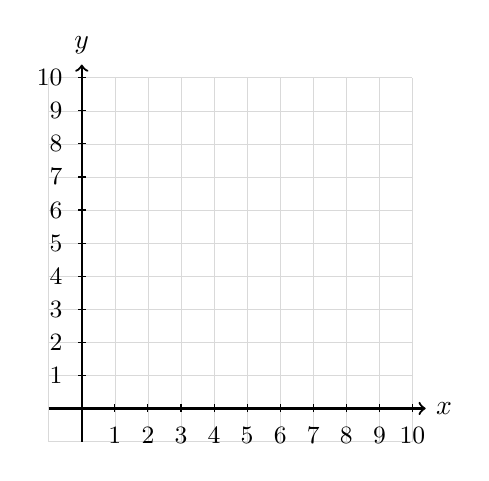
\begin{tikzpicture}[scale=0.42]
    \draw[step=1cm,gray!30,very thin] (-1,-1) grid (10,10);
    \draw[->,thick] (-1,0)--(10.4,0) node[right] {$x$};
    \draw[->,thick] (0,-1)--(0,10.4) node[above] {$y$};
    \foreach \x in {1,...,10} \draw (\x,0.12)--(\x,-0.12) node[below=2pt] {\small\x};
    \foreach \y in {1,...,10} \draw (0.12,\y)--(-0.12,\y) node[left=2pt] {\small\y};
  \end{tikzpicture}
  \end{center}

  \item Let
  \[
    r(x)=2(x+1)^3-5.
  \]
  Find $r^{-1}(x)$. Then verify algebraically that
  \[
    r(r^{-1}(x))=x
    \qquad\text{and}\qquad
    r^{-1}(r(x))=x.
  \]
  State what these two identities mean about the input-output actions of inverse functions.
\end{enumerate}

\end{document}
